\documentclass[pdftex,12pt,a4paper]{report}

\usepackage[pdftex]{graphicx}
\usepackage{float}
\usepackage{fancyvrb}
\fvset{xleftmargin=2em}
\usepackage{multicol}
\usepackage{wrapfig}
\usepackage[official]{eurosym}
\usepackage{indentfirst}

\usepackage{pgfplots}
\pgfplotsset{width=10cm,compat=1.9}
\usepackage{tikzscale}
\usepackage{pgfplotstable}
\usepackage{booktabs}
\usepackage[font=small,labelfont=bf,tableposition=top]{caption}


\usepackage[utf8]{inputenc} % isto é um comentário
\usepackage[portuges]{babel}
\usepackage[T1]{fontenc}
\usepackage{times}
%\usepackage{lmodern}
\usepackage[obeyspaces,spaces]{url}
\usepackage[left=15mm,right=15mm,top=10mm,bottom=10mm]{geometry}
\usepackage{titlesec}
\usepackage{mathtools}
%identa 1º paragrafo de capitulos e secções
\usepackage{indentfirst}

\newcommand{\HRule}{\rule{\linewidth}{0.5mm}}
\titleformat{\chapter}{\normalfont\huge}{\thechapter.}{20pt}{\huge}


\begin{document}

\begin{titlepage}


\begin{minipage}{0.3\textwidth}
\begin{flushleft} 

\includegraphics[width=\textwidth]{logo.png}
\end{flushleft}
\end{minipage}
\begin{minipage}{0.6\textwidth}
\begin{flushright} 

\textsc{Departamento de Produção de Sistemas}\\[0.1cm]
\bfseries Mestrado em Engenharia de Sistemas\\ [0.1cm]
\bfseries \textit{Logística}\\[8mm]

\end{flushright}
\end{minipage}


\vspace{3cm}


\begin{center}


\LARGE Relatório

\vspace{1cm}
\huge \textbf{\textit{"The Beer game"}}\\[1.5cm]


\noindent\begin{minipage}[b]{.2\textwidth}
	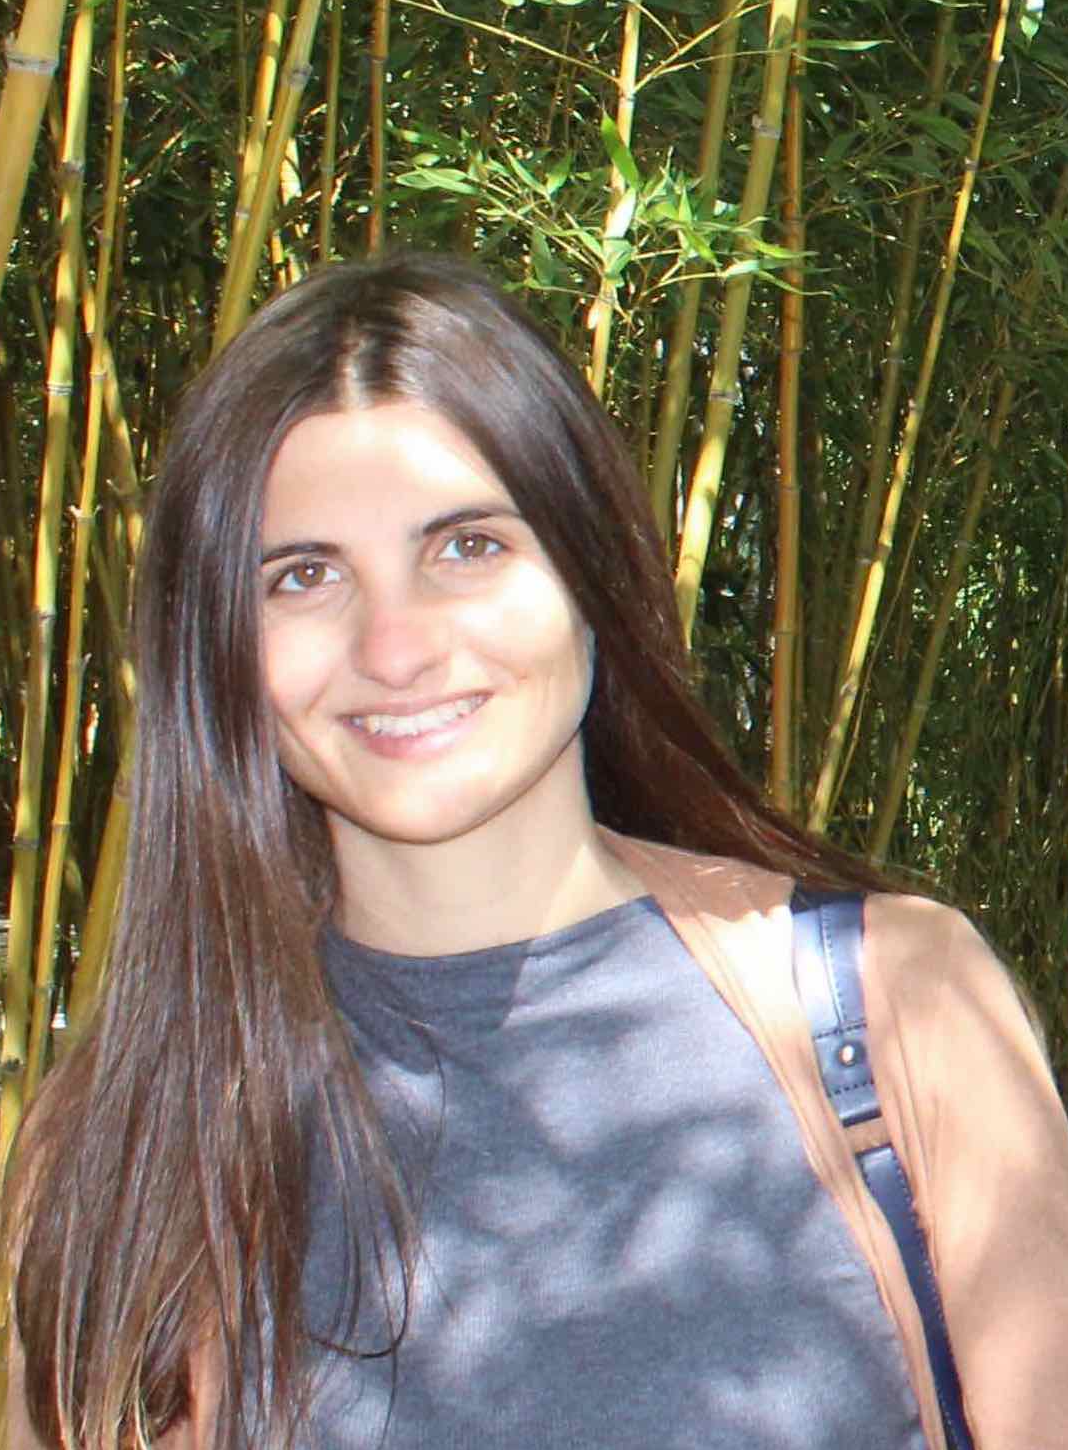
\includegraphics[scale=0.09]{celia}
	\small{Célia Figueiredo a67637}
\end{minipage} 
\hfill
\begin{minipage}[b]{.2\textwidth}
	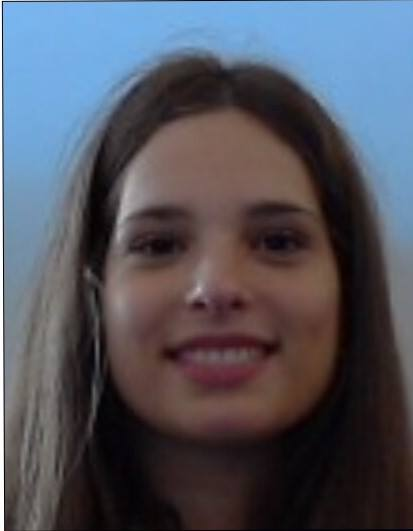
\includegraphics[scale=0.239]{carolina}
	\small{Carolina Silva  pg38335}
\end{minipage}
\hfill
\begin{minipage}[b]{.2\textwidth}
	
\includegraphics[scale=0.15]{marcia}
	\small{Márcia Costa a67672}
\end{minipage}
\hfill
\begin{minipage}[b]{.2\textwidth}
	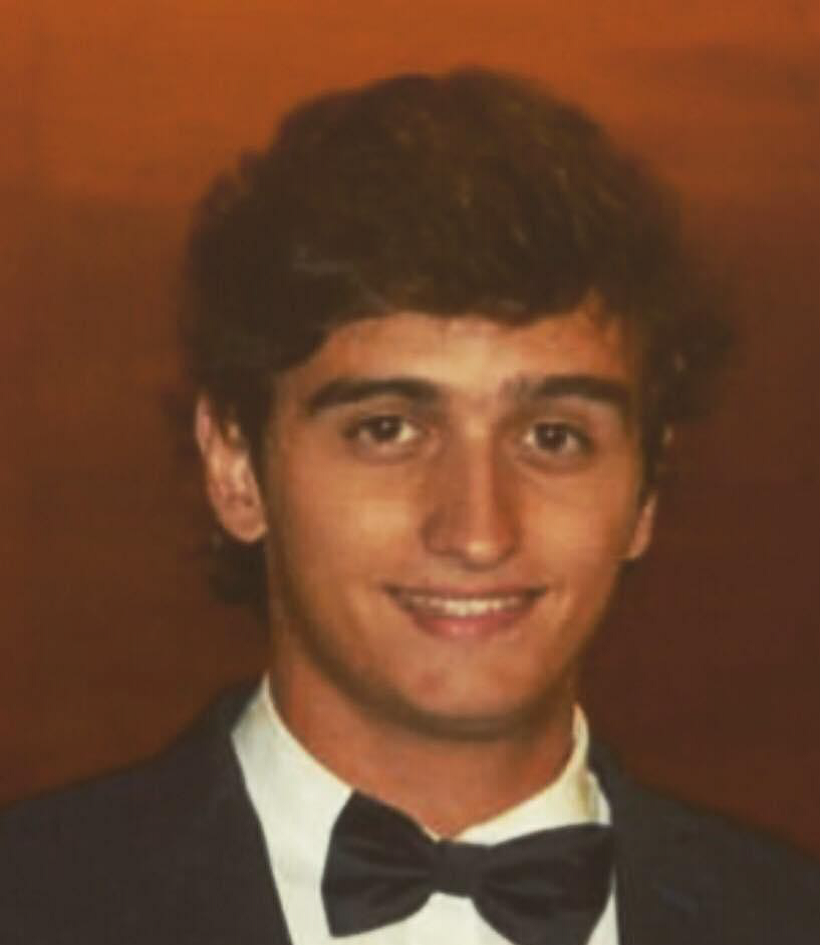
\includegraphics[scale=0.136]{luispedro}
	\small{Luis Pedro Freitas pg38347}
\end{minipage}




\vspace{3ex}


\vfill

\large Braga, {\large \today}

\end{center}
\end{titlepage}


\tableofcontents
%\input{chapters/resumo}
\chapter{Introdução}
\label{cap:intro}

O presente relatório documenta uma análise de resultados, resultantes da simulação de  uma cadeia de abastecimento de cerveja. Reproduziu-se o comportamento de um sistema de produção e distribuição de grades de cerveja com o objetivo de ensaiar políticas alternativas de gestão da cadeia de abastecimento. 

\chapter{Descrição geral do projeto}
\section{Cadeia de Abastecimento de Cerveja}


O projeto consiste na simulação e análise de uma cadeia de abastecimento de cerveja e foi didivido em duas fases. A primeira fase consistiu em formar vários grupos de alunos, em que cada um dos grupos representava uma cadeia de abastecimento e o cliente seria representado pela docente. Formando uma cadeia de abastecimento com a seguinte estrutura: 

\begin{figure}[tbph]
	\centering
	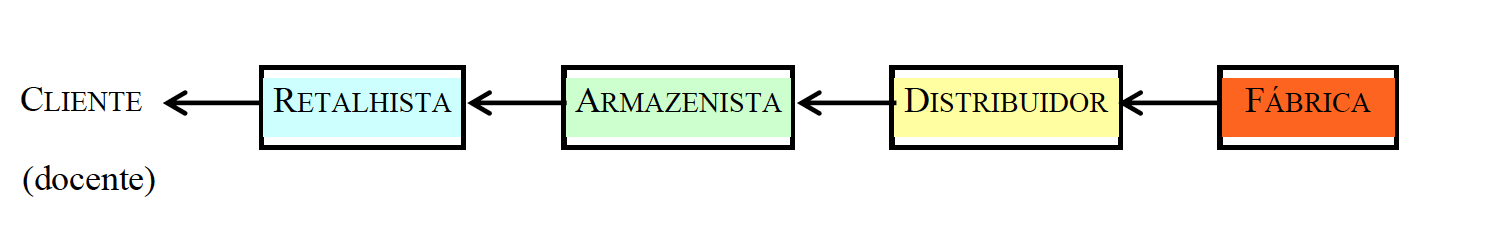
\includegraphics[scale=0.5]{imagem/estrutura.png}
	\caption{Estrutura da cadeia de abastecimento}
	\label{fig:cominicacaoservidorcliente}
\end{figure}

Ao longo da simulação, cada equipa teria apenas conhecimento das encomendas que de semana a semana a equipa localizada a jusante vai pedindo. Com base nesta informação cada equipa deverá encontrar um algoritmo de gestão de stock, de modo a satisfazer os pedidos do cliente, e obter o melhor desempenho possível em termos de custo total de operação no final de todo o processo. O prazo establecido para a entrega de todas as encomendas é de 2 semanas. 

Para o cálculo de atualização do registo interno do inventário usaram-se as seguintes fórmulas: 

$emTransito1(t) = emTransito2(t-1)$

$stockAbertura (t) = stockFecho(t-1) + emTransito1(t-1)$

$despacho = min [(pedido + porDespachar); stockAbertura]$

$porDespachar(t) = porDespachar(t -1) + [pedido(t) - despacho(t)]$

$stockFecho = stockAbertura - despacho $
\vspace{1cm}

Os custos associados serão: 
\begin{itemize}
	\item Custo de posse = 1\euro/artigo/semana
	\item Custo de quebra = 2\euro/artigo/semana 
	\item Custo de encomenda = 5\euro/encomenda 
	\item Custo de produção = 5\euro   (apenas na Fábrica)
\end{itemize}




\chapter{Análise de Resultados}
\section{Cálculo dos custos de operação}

\subsection{Custo de Produção}
Inicialmente ficou definido que o custo de produção seria de 5\euro{}  por encomenda, o prazo de entrega seria de duas semanas e o pagamento será efetuado no momento da encomenda. Portanto para o cálculo do custo de produção na fábrica utilizou-se a seguinte 

\subsection{Custo de Posse}



\subsection{Custo de Quebra}

\subsection{Custo de Encomenda}


\section{Análise da evolução dos níveis de stock e roturas}


\chapter{Limitações ao desempenho da cadeia}







\chapter{Melhorias/Sugestões de desempenho }







\chapter{Conclusões }

Com a realização desta análise 

\end {document}


